% Created by tikzDevice version 0.12.3.2 on 2021-12-07 15:43:52
% !TEX encoding = UTF-8 Unicode
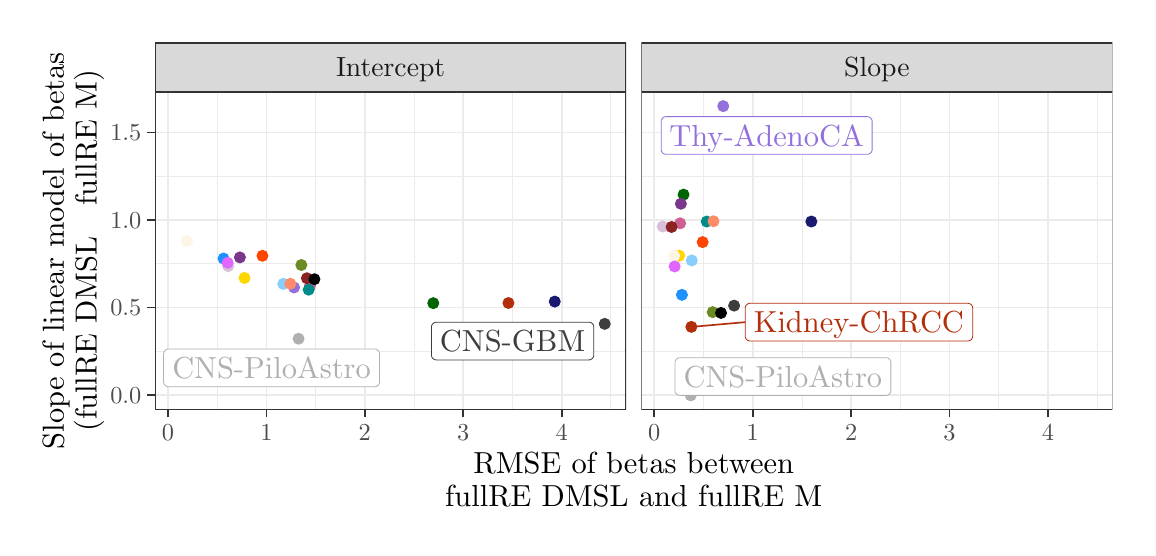
\begin{tikzpicture}[x=1pt,y=1pt]
\definecolor{fillColor}{RGB}{255,255,255}
\path[use as bounding box,fill=fillColor,fill opacity=0.00] (0,0) rectangle (397.48,180.67);
\begin{scope}
\path[clip] (  0.00,  0.00) rectangle (397.48,180.67);
\definecolor{drawColor}{RGB}{255,255,255}
\definecolor{fillColor}{RGB}{255,255,255}

\path[draw=drawColor,line width= 0.6pt,line join=round,line cap=round,fill=fillColor] (  0.00,  0.00) rectangle (397.48,180.68);
\end{scope}
\begin{scope}
\path[clip] ( 46.04, 42.57) rectangle (216.26,157.54);
\definecolor{fillColor}{RGB}{255,255,255}

\path[fill=fillColor] ( 46.04, 42.57) rectangle (216.26,157.54);
\definecolor{drawColor}{gray}{0.92}

\path[draw=drawColor,line width= 0.3pt,line join=round] ( 46.04, 63.75) --
	(216.26, 63.75);

\path[draw=drawColor,line width= 0.3pt,line join=round] ( 46.04, 95.36) --
	(216.26, 95.36);

\path[draw=drawColor,line width= 0.3pt,line join=round] ( 46.04,126.98) --
	(216.26,126.98);

\path[draw=drawColor,line width= 0.3pt,line join=round] ( 68.49, 42.57) --
	( 68.49,157.54);

\path[draw=drawColor,line width= 0.3pt,line join=round] (104.05, 42.57) --
	(104.05,157.54);

\path[draw=drawColor,line width= 0.3pt,line join=round] (139.62, 42.57) --
	(139.62,157.54);

\path[draw=drawColor,line width= 0.3pt,line join=round] (175.18, 42.57) --
	(175.18,157.54);

\path[draw=drawColor,line width= 0.3pt,line join=round] (210.74, 42.57) --
	(210.74,157.54);

\path[draw=drawColor,line width= 0.6pt,line join=round] ( 46.04, 47.94) --
	(216.26, 47.94);

\path[draw=drawColor,line width= 0.6pt,line join=round] ( 46.04, 79.55) --
	(216.26, 79.55);

\path[draw=drawColor,line width= 0.6pt,line join=round] ( 46.04,111.17) --
	(216.26,111.17);

\path[draw=drawColor,line width= 0.6pt,line join=round] ( 46.04,142.79) --
	(216.26,142.79);

\path[draw=drawColor,line width= 0.6pt,line join=round] ( 50.70, 42.57) --
	( 50.70,157.54);

\path[draw=drawColor,line width= 0.6pt,line join=round] ( 86.27, 42.57) --
	( 86.27,157.54);

\path[draw=drawColor,line width= 0.6pt,line join=round] (121.83, 42.57) --
	(121.83,157.54);

\path[draw=drawColor,line width= 0.6pt,line join=round] (157.40, 42.57) --
	(157.40,157.54);

\path[draw=drawColor,line width= 0.6pt,line join=round] (192.96, 42.57) --
	(192.96,157.54);
\definecolor{drawColor}{RGB}{255,215,0}
\definecolor{fillColor}{RGB}{255,215,0}

\path[draw=drawColor,line width= 0.4pt,line join=round,line cap=round,fill=fillColor] ( 78.35, 90.23) circle (  1.96);
\definecolor{drawColor}{RGB}{205,96,144}
\definecolor{fillColor}{RGB}{205,96,144}

\path[draw=drawColor,line width= 0.4pt,line join=round,line cap=round,fill=fillColor] (102.06, 87.52) circle (  1.96);
\definecolor{drawColor}{gray}{0.24}
\definecolor{fillColor}{gray}{0.24}

\path[draw=drawColor,line width= 0.4pt,line join=round,line cap=round,fill=fillColor] (208.52, 73.64) circle (  1.96);
\definecolor{drawColor}{RGB}{216,191,216}
\definecolor{fillColor}{RGB}{216,191,216}

\path[draw=drawColor,line width= 0.4pt,line join=round,line cap=round,fill=fillColor] ( 72.44, 94.52) circle (  1.96);
\definecolor{drawColor}{gray}{0.69}
\definecolor{fillColor}{gray}{0.69}

\path[draw=drawColor,line width= 0.4pt,line join=round,line cap=round,fill=fillColor] ( 97.88, 68.27) circle (  1.96);
\definecolor{drawColor}{RGB}{25,25,112}
\definecolor{fillColor}{RGB}{25,25,112}

\path[draw=drawColor,line width= 0.4pt,line join=round,line cap=round,fill=fillColor] (190.46, 81.69) circle (  1.96);
\definecolor{drawColor}{RGB}{30,144,255}
\definecolor{fillColor}{RGB}{30,144,255}

\path[draw=drawColor,line width= 0.4pt,line join=round,line cap=round,fill=fillColor] ( 70.78, 97.25) circle (  1.96);
\definecolor{drawColor}{RGB}{139,35,35}
\definecolor{fillColor}{RGB}{139,35,35}

\path[draw=drawColor,line width= 0.4pt,line join=round,line cap=round,fill=fillColor] (100.90, 90.13) circle (  1.96);
\definecolor{drawColor}{RGB}{179,47,11}
\definecolor{fillColor}{RGB}{179,47,11}

\path[draw=drawColor,line width= 0.4pt,line join=round,line cap=round,fill=fillColor] (173.72, 81.18) circle (  1.96);
\definecolor{drawColor}{RGB}{255,69,0}
\definecolor{fillColor}{RGB}{255,69,0}

\path[draw=drawColor,line width= 0.4pt,line join=round,line cap=round,fill=fillColor] ( 84.83, 98.23) circle (  1.96);
\definecolor{drawColor}{RGB}{0,100,0}
\definecolor{fillColor}{RGB}{0,100,0}

\path[draw=drawColor,line width= 0.4pt,line join=round,line cap=round,fill=fillColor] (146.56, 81.12) circle (  1.96);
\definecolor{drawColor}{RGB}{253,245,230}
\definecolor{fillColor}{RGB}{253,245,230}

\path[draw=drawColor,line width= 0.4pt,line join=round,line cap=round,fill=fillColor] ( 57.55,103.56) circle (  1.96);
\definecolor{drawColor}{RGB}{105,139,34}
\definecolor{fillColor}{RGB}{105,139,34}

\path[draw=drawColor,line width= 0.4pt,line join=round,line cap=round,fill=fillColor] ( 98.89, 94.91) circle (  1.96);
\definecolor{drawColor}{RGB}{0,139,139}
\definecolor{fillColor}{RGB}{0,139,139}

\path[draw=drawColor,line width= 0.4pt,line join=round,line cap=round,fill=fillColor] (101.54, 85.99) circle (  1.96);
\definecolor{drawColor}{RGB}{122,55,139}
\definecolor{fillColor}{RGB}{122,55,139}

\path[draw=drawColor,line width= 0.4pt,line join=round,line cap=round,fill=fillColor] ( 76.69, 97.66) circle (  1.96);
\definecolor{drawColor}{RGB}{224,102,255}
\definecolor{fillColor}{RGB}{224,102,255}

\path[draw=drawColor,line width= 0.4pt,line join=round,line cap=round,fill=fillColor] ( 72.26, 95.71) circle (  1.96);
\definecolor{drawColor}{RGB}{135,206,250}
\definecolor{fillColor}{RGB}{135,206,250}

\path[draw=drawColor,line width= 0.4pt,line join=round,line cap=round,fill=fillColor] ( 92.37, 88.09) circle (  1.96);
\definecolor{drawColor}{RGB}{0,0,0}
\definecolor{fillColor}{RGB}{0,0,0}

\path[draw=drawColor,line width= 0.4pt,line join=round,line cap=round,fill=fillColor] (103.61, 89.78) circle (  1.96);
\definecolor{drawColor}{RGB}{147,112,219}
\definecolor{fillColor}{RGB}{147,112,219}

\path[draw=drawColor,line width= 0.4pt,line join=round,line cap=round,fill=fillColor] ( 96.25, 86.78) circle (  1.96);
\definecolor{drawColor}{RGB}{255,140,105}
\definecolor{fillColor}{RGB}{255,140,105}

\path[draw=drawColor,line width= 0.4pt,line join=round,line cap=round,fill=fillColor] ( 94.91, 88.14) circle (  1.96);
\end{scope}
\begin{scope}
\path[clip] ( 46.04, 42.57) rectangle (216.26,157.54);
\definecolor{drawColor}{gray}{0.24}
\definecolor{fillColor}{RGB}{255,255,255}

\path[draw=drawColor,line width= 0.3pt,line join=round,line cap=round,fill=fillColor] (147.70, 60.61) --
	(202.77, 60.61) --
	(202.69, 60.62) --
	(202.98, 60.63) --
	(203.27, 60.69) --
	(203.54, 60.79) --
	(203.79, 60.93) --
	(204.02, 61.12) --
	(204.21, 61.34) --
	(204.37, 61.58) --
	(204.48, 61.85) --
	(204.55, 62.13) --
	(204.57, 62.42) --
	(204.57, 62.42) --
	(204.57, 72.43) --
	(204.57, 72.43) --
	(204.55, 72.72) --
	(204.48, 73.01) --
	(204.37, 73.27) --
	(204.21, 73.52) --
	(204.02, 73.74) --
	(203.79, 73.92) --
	(203.54, 74.07) --
	(203.27, 74.17) --
	(202.98, 74.23) --
	(202.77, 74.24) --
	(147.70, 74.24) --
	(147.92, 74.23) --
	(147.63, 74.24) --
	(147.34, 74.20) --
	(147.06, 74.12) --
	(146.80, 74.00) --
	(146.56, 73.83) --
	(146.35, 73.63) --
	(146.17, 73.40) --
	(146.04, 73.14) --
	(145.94, 72.87) --
	(145.90, 72.58) --
	(145.89, 72.43) --
	(145.89, 62.42) --
	(145.90, 62.57) --
	(145.90, 62.28) --
	(145.94, 61.99) --
	(146.04, 61.71) --
	(146.17, 61.46) --
	(146.35, 61.22) --
	(146.56, 61.02) --
	(146.80, 60.86) --
	(147.06, 60.73) --
	(147.34, 60.65) --
	(147.63, 60.62) --
	cycle;
\end{scope}
\begin{scope}
\path[clip] ( 46.04, 42.57) rectangle (216.26,157.54);
\definecolor{drawColor}{gray}{0.24}

\node[text=drawColor,anchor=base,inner sep=0pt, outer sep=0pt, scale=  1.10] at (175.23, 63.63) {CNS-GBM};
\definecolor{drawColor}{gray}{0.69}
\definecolor{fillColor}{RGB}{255,255,255}

\path[draw=drawColor,line width= 0.3pt,line join=round,line cap=round,fill=fillColor] ( 50.92, 50.91) --
	(125.32, 50.91) --
	(125.24, 50.91) --
	(125.53, 50.93) --
	(125.82, 50.98) --
	(126.09, 51.09) --
	(126.34, 51.23) --
	(126.57, 51.42) --
	(126.76, 51.63) --
	(126.92, 51.88) --
	(127.03, 52.15) --
	(127.10, 52.43) --
	(127.12, 52.72) --
	(127.12, 52.72) --
	(127.12, 62.73) --
	(127.12, 62.73) --
	(127.10, 63.02) --
	(127.03, 63.30) --
	(126.92, 63.57) --
	(126.76, 63.82) --
	(126.57, 64.03) --
	(126.34, 64.22) --
	(126.09, 64.36) --
	(125.82, 64.47) --
	(125.53, 64.53) --
	(125.32, 64.54) --
	( 50.92, 64.54) --
	( 51.14, 64.53) --
	( 50.85, 64.54) --
	( 50.56, 64.50) --
	( 50.28, 64.42) --
	( 50.02, 64.30) --
	( 49.78, 64.13) --
	( 49.57, 63.93) --
	( 49.39, 63.70) --
	( 49.26, 63.44) --
	( 49.17, 63.16) --
	( 49.12, 62.88) --
	( 49.11, 62.73) --
	( 49.11, 52.72) --
	( 49.12, 52.86) --
	( 49.12, 52.57) --
	( 49.17, 52.29) --
	( 49.26, 52.01) --
	( 49.39, 51.75) --
	( 49.57, 51.52) --
	( 49.78, 51.32) --
	( 50.02, 51.15) --
	( 50.28, 51.03) --
	( 50.56, 50.95) --
	( 50.85, 50.91) --
	cycle;
\end{scope}
\begin{scope}
\path[clip] ( 46.04, 42.57) rectangle (216.26,157.54);
\definecolor{drawColor}{gray}{0.69}

\node[text=drawColor,anchor=base,inner sep=0pt, outer sep=0pt, scale=  1.10] at ( 88.12, 53.92) {CNS-PiloAstro};
\definecolor{drawColor}{gray}{0.20}

\path[draw=drawColor,line width= 0.6pt,line join=round,line cap=round] ( 46.04, 42.57) rectangle (216.26,157.54);
\end{scope}
\begin{scope}
\path[clip] (221.76, 42.57) rectangle (391.98,157.54);
\definecolor{fillColor}{RGB}{255,255,255}

\path[fill=fillColor] (221.76, 42.57) rectangle (391.98,157.54);
\definecolor{drawColor}{gray}{0.92}

\path[draw=drawColor,line width= 0.3pt,line join=round] (221.76, 63.75) --
	(391.98, 63.75);

\path[draw=drawColor,line width= 0.3pt,line join=round] (221.76, 95.36) --
	(391.98, 95.36);

\path[draw=drawColor,line width= 0.3pt,line join=round] (221.76,126.98) --
	(391.98,126.98);

\path[draw=drawColor,line width= 0.3pt,line join=round] (244.21, 42.57) --
	(244.21,157.54);

\path[draw=drawColor,line width= 0.3pt,line join=round] (279.78, 42.57) --
	(279.78,157.54);

\path[draw=drawColor,line width= 0.3pt,line join=round] (315.34, 42.57) --
	(315.34,157.54);

\path[draw=drawColor,line width= 0.3pt,line join=round] (350.90, 42.57) --
	(350.90,157.54);

\path[draw=drawColor,line width= 0.3pt,line join=round] (386.47, 42.57) --
	(386.47,157.54);

\path[draw=drawColor,line width= 0.6pt,line join=round] (221.76, 47.94) --
	(391.98, 47.94);

\path[draw=drawColor,line width= 0.6pt,line join=round] (221.76, 79.55) --
	(391.98, 79.55);

\path[draw=drawColor,line width= 0.6pt,line join=round] (221.76,111.17) --
	(391.98,111.17);

\path[draw=drawColor,line width= 0.6pt,line join=round] (221.76,142.79) --
	(391.98,142.79);

\path[draw=drawColor,line width= 0.6pt,line join=round] (226.43, 42.57) --
	(226.43,157.54);

\path[draw=drawColor,line width= 0.6pt,line join=round] (261.99, 42.57) --
	(261.99,157.54);

\path[draw=drawColor,line width= 0.6pt,line join=round] (297.56, 42.57) --
	(297.56,157.54);

\path[draw=drawColor,line width= 0.6pt,line join=round] (333.12, 42.57) --
	(333.12,157.54);

\path[draw=drawColor,line width= 0.6pt,line join=round] (368.69, 42.57) --
	(368.69,157.54);
\definecolor{drawColor}{RGB}{255,215,0}
\definecolor{fillColor}{RGB}{255,215,0}

\path[draw=drawColor,line width= 0.4pt,line join=round,line cap=round,fill=fillColor] (235.45, 98.28) circle (  1.96);
\definecolor{drawColor}{RGB}{205,96,144}
\definecolor{fillColor}{RGB}{205,96,144}

\path[draw=drawColor,line width= 0.4pt,line join=round,line cap=round,fill=fillColor] (235.76,109.98) circle (  1.96);
\definecolor{drawColor}{gray}{0.24}
\definecolor{fillColor}{gray}{0.24}

\path[draw=drawColor,line width= 0.4pt,line join=round,line cap=round,fill=fillColor] (255.27, 80.23) circle (  1.96);
\definecolor{drawColor}{RGB}{216,191,216}
\definecolor{fillColor}{RGB}{216,191,216}

\path[draw=drawColor,line width= 0.4pt,line join=round,line cap=round,fill=fillColor] (229.50,108.81) circle (  1.96);
\definecolor{drawColor}{gray}{0.69}
\definecolor{fillColor}{gray}{0.69}

\path[draw=drawColor,line width= 0.4pt,line join=round,line cap=round,fill=fillColor] (239.60, 47.79) circle (  1.96);
\definecolor{drawColor}{RGB}{25,25,112}
\definecolor{fillColor}{RGB}{25,25,112}

\path[draw=drawColor,line width= 0.4pt,line join=round,line cap=round,fill=fillColor] (283.18,110.62) circle (  1.96);
\definecolor{drawColor}{RGB}{30,144,255}
\definecolor{fillColor}{RGB}{30,144,255}

\path[draw=drawColor,line width= 0.4pt,line join=round,line cap=round,fill=fillColor] (236.41, 84.13) circle (  1.96);
\definecolor{drawColor}{RGB}{139,35,35}
\definecolor{fillColor}{RGB}{139,35,35}

\path[draw=drawColor,line width= 0.4pt,line join=round,line cap=round,fill=fillColor] (232.68,108.65) circle (  1.96);
\definecolor{drawColor}{RGB}{179,47,11}
\definecolor{fillColor}{RGB}{179,47,11}

\path[draw=drawColor,line width= 0.4pt,line join=round,line cap=round,fill=fillColor] (239.82, 72.55) circle (  1.96);
\definecolor{drawColor}{RGB}{255,69,0}
\definecolor{fillColor}{RGB}{255,69,0}

\path[draw=drawColor,line width= 0.4pt,line join=round,line cap=round,fill=fillColor] (243.90,103.18) circle (  1.96);
\definecolor{drawColor}{RGB}{0,100,0}
\definecolor{fillColor}{RGB}{0,100,0}

\path[draw=drawColor,line width= 0.4pt,line join=round,line cap=round,fill=fillColor] (237.00,120.34) circle (  1.96);
\definecolor{drawColor}{RGB}{253,245,230}
\definecolor{fillColor}{RGB}{253,245,230}

\path[draw=drawColor,line width= 0.4pt,line join=round,line cap=round,fill=fillColor] (233.62, 98.21) circle (  1.96);
\definecolor{drawColor}{RGB}{105,139,34}
\definecolor{fillColor}{RGB}{105,139,34}

\path[draw=drawColor,line width= 0.4pt,line join=round,line cap=round,fill=fillColor] (247.52, 77.89) circle (  1.96);
\definecolor{drawColor}{RGB}{0,139,139}
\definecolor{fillColor}{RGB}{0,139,139}

\path[draw=drawColor,line width= 0.4pt,line join=round,line cap=round,fill=fillColor] (245.37,110.61) circle (  1.96);
\definecolor{drawColor}{RGB}{122,55,139}
\definecolor{fillColor}{RGB}{122,55,139}

\path[draw=drawColor,line width= 0.4pt,line join=round,line cap=round,fill=fillColor] (236.03,117.04) circle (  1.96);
\definecolor{drawColor}{RGB}{224,102,255}
\definecolor{fillColor}{RGB}{224,102,255}

\path[draw=drawColor,line width= 0.4pt,line join=round,line cap=round,fill=fillColor] (233.78, 94.38) circle (  1.96);
\definecolor{drawColor}{RGB}{135,206,250}
\definecolor{fillColor}{RGB}{135,206,250}

\path[draw=drawColor,line width= 0.4pt,line join=round,line cap=round,fill=fillColor] (239.97, 96.56) circle (  1.96);
\definecolor{drawColor}{RGB}{0,0,0}
\definecolor{fillColor}{RGB}{0,0,0}

\path[draw=drawColor,line width= 0.4pt,line join=round,line cap=round,fill=fillColor] (250.54, 77.59) circle (  1.96);
\definecolor{drawColor}{RGB}{147,112,219}
\definecolor{fillColor}{RGB}{147,112,219}

\path[draw=drawColor,line width= 0.4pt,line join=round,line cap=round,fill=fillColor] (251.33,152.32) circle (  1.96);
\definecolor{drawColor}{RGB}{255,140,105}
\definecolor{fillColor}{RGB}{255,140,105}

\path[draw=drawColor,line width= 0.4pt,line join=round,line cap=round,fill=fillColor] (247.82,110.72) circle (  1.96);
\end{scope}
\begin{scope}
\path[clip] (221.76, 42.57) rectangle (391.98,157.54);
\definecolor{drawColor}{RGB}{179,47,11}

\path[draw=drawColor,line width= 0.6pt,line join=round,line cap=round] (259.27, 74.25) -- (240.98, 72.65);
\definecolor{drawColor}{gray}{0.69}
\definecolor{fillColor}{RGB}{255,255,255}

\path[draw=drawColor,line width= 0.3pt,line join=round,line cap=round,fill=fillColor] (235.70, 47.80) --
	(310.10, 47.80) --
	(310.03, 47.80) --
	(310.32, 47.81) --
	(310.60, 47.87) --
	(310.88, 47.97) --
	(311.13, 48.12) --
	(311.35, 48.30) --
	(311.55, 48.52) --
	(311.70, 48.77) --
	(311.82, 49.03) --
	(311.89, 49.32) --
	(311.91, 49.61) --
	(311.91, 49.61) --
	(311.91, 59.62) --
	(311.91, 59.62) --
	(311.89, 59.91) --
	(311.82, 60.19) --
	(311.70, 60.46) --
	(311.55, 60.70) --
	(311.35, 60.92) --
	(311.13, 61.10) --
	(310.88, 61.25) --
	(310.60, 61.35) --
	(310.32, 61.41) --
	(310.10, 61.42) --
	(235.70, 61.42) --
	(235.92, 61.41) --
	(235.63, 61.42) --
	(235.34, 61.39) --
	(235.06, 61.31) --
	(234.80, 61.18) --
	(234.56, 61.02) --
	(234.35, 60.82) --
	(234.18, 60.58) --
	(234.04, 60.33) --
	(233.95, 60.05) --
	(233.90, 59.76) --
	(233.90, 59.62) --
	(233.90, 49.61) --
	(233.90, 49.75) --
	(233.90, 49.46) --
	(233.95, 49.17) --
	(234.04, 48.90) --
	(234.18, 48.64) --
	(234.35, 48.41) --
	(234.56, 48.21) --
	(234.80, 48.04) --
	(235.06, 47.92) --
	(235.34, 47.84) --
	(235.63, 47.80) --
	cycle;
\end{scope}
\begin{scope}
\path[clip] (221.76, 42.57) rectangle (391.98,157.54);
\definecolor{drawColor}{gray}{0.69}

\node[text=drawColor,anchor=base,inner sep=0pt, outer sep=0pt, scale=  1.10] at (272.90, 50.81) {CNS-PiloAstro};
\definecolor{drawColor}{RGB}{179,47,11}
\definecolor{fillColor}{RGB}{255,255,255}

\path[draw=drawColor,line width= 0.3pt,line join=round,line cap=round,fill=fillColor] (261.08, 67.45) --
	(339.67, 67.45) --
	(339.60, 67.45) --
	(339.89, 67.46) --
	(340.18, 67.52) --
	(340.45, 67.62) --
	(340.70, 67.77) --
	(340.93, 67.95) --
	(341.12, 68.17) --
	(341.27, 68.42) --
	(341.39, 68.68) --
	(341.46, 68.97) --
	(341.48, 69.26) --
	(341.48, 69.26) --
	(341.48, 79.27) --
	(341.48, 79.27) --
	(341.46, 79.56) --
	(341.39, 79.84) --
	(341.27, 80.11) --
	(341.12, 80.35) --
	(340.93, 80.57) --
	(340.70, 80.75) --
	(340.45, 80.90) --
	(340.18, 81.00) --
	(339.89, 81.06) --
	(339.67, 81.07) --
	(261.08, 81.07) --
	(261.29, 81.06) --
	(261.00, 81.07) --
	(260.71, 81.04) --
	(260.44, 80.96) --
	(260.17, 80.83) --
	(259.93, 80.67) --
	(259.72, 80.47) --
	(259.55, 80.23) --
	(259.41, 79.98) --
	(259.32, 79.70) --
	(259.28, 79.41) --
	(259.27, 79.27) --
	(259.27, 69.26) --
	(259.28, 69.40) --
	(259.28, 69.11) --
	(259.32, 68.82) --
	(259.41, 68.55) --
	(259.55, 68.29) --
	(259.72, 68.06) --
	(259.93, 67.86) --
	(260.17, 67.69) --
	(260.44, 67.57) --
	(260.71, 67.48) --
	(261.00, 67.45) --
	cycle;
\end{scope}
\begin{scope}
\path[clip] (221.76, 42.57) rectangle (391.98,157.54);
\definecolor{drawColor}{RGB}{179,47,11}

\node[text=drawColor,anchor=base,inner sep=0pt, outer sep=0pt, scale=  1.10] at (300.37, 70.46) {Kidney-ChRCC};
\definecolor{drawColor}{RGB}{147,112,219}
\definecolor{fillColor}{RGB}{255,255,255}

\path[draw=drawColor,line width= 0.3pt,line join=round,line cap=round,fill=fillColor] (230.72,134.90) --
	(303.34,134.90) --
	(303.27,134.90) --
	(303.56,134.91) --
	(303.84,134.97) --
	(304.12,135.07) --
	(304.37,135.22) --
	(304.59,135.40) --
	(304.79,135.62) --
	(304.94,135.86) --
	(305.06,136.13) --
	(305.13,136.41) --
	(305.15,136.70) --
	(305.15,136.70) --
	(305.15,146.72) --
	(305.15,146.72) --
	(305.13,147.01) --
	(305.06,147.29) --
	(304.94,147.56) --
	(304.79,147.80) --
	(304.59,148.02) --
	(304.37,148.20) --
	(304.12,148.35) --
	(303.84,148.45) --
	(303.56,148.51) --
	(303.34,148.52) --
	(230.72,148.52) --
	(230.94,148.51) --
	(230.65,148.52) --
	(230.36,148.49) --
	(230.08,148.41) --
	(229.82,148.28) --
	(229.58,148.12) --
	(229.37,147.91) --
	(229.20,147.68) --
	(229.06,147.42) --
	(228.97,147.15) --
	(228.92,146.86) --
	(228.92,146.72) --
	(228.92,136.70) --
	(228.92,136.85) --
	(228.92,136.56) --
	(228.97,136.27) --
	(229.06,136.00) --
	(229.20,135.74) --
	(229.37,135.51) --
	(229.58,135.30) --
	(229.82,135.14) --
	(230.08,135.01) --
	(230.36,134.93) --
	(230.65,134.90) --
	cycle;
\end{scope}
\begin{scope}
\path[clip] (221.76, 42.57) rectangle (391.98,157.54);
\definecolor{drawColor}{RGB}{147,112,219}

\node[text=drawColor,anchor=base,inner sep=0pt, outer sep=0pt, scale=  1.10] at (267.03,137.91) {Thy-AdenoCA};
\definecolor{drawColor}{gray}{0.20}

\path[draw=drawColor,line width= 0.6pt,line join=round,line cap=round] (221.76, 42.57) rectangle (391.98,157.54);
\end{scope}
\begin{scope}
\path[clip] ( 46.04,157.54) rectangle (216.26,175.17);
\definecolor{drawColor}{gray}{0.20}
\definecolor{fillColor}{gray}{0.85}

\path[draw=drawColor,line width= 0.6pt,line join=round,line cap=round,fill=fillColor] ( 46.04,157.54) rectangle (216.26,175.17);
\definecolor{drawColor}{gray}{0.10}

\node[text=drawColor,anchor=base,inner sep=0pt, outer sep=0pt, scale=  1.00] at (131.15,162.92) {Intercept};
\end{scope}
\begin{scope}
\path[clip] (221.76,157.54) rectangle (391.98,175.17);
\definecolor{drawColor}{gray}{0.20}
\definecolor{fillColor}{gray}{0.85}

\path[draw=drawColor,line width= 0.6pt,line join=round,line cap=round,fill=fillColor] (221.76,157.54) rectangle (391.98,175.17);
\definecolor{drawColor}{gray}{0.10}

\node[text=drawColor,anchor=base,inner sep=0pt, outer sep=0pt, scale=  1.00] at (306.87,162.92) {Slope};
\end{scope}
\begin{scope}
\path[clip] (  0.00,  0.00) rectangle (397.48,180.67);
\definecolor{drawColor}{gray}{0.20}

\path[draw=drawColor,line width= 0.6pt,line join=round] ( 50.70, 39.82) --
	( 50.70, 42.57);

\path[draw=drawColor,line width= 0.6pt,line join=round] ( 86.27, 39.82) --
	( 86.27, 42.57);

\path[draw=drawColor,line width= 0.6pt,line join=round] (121.83, 39.82) --
	(121.83, 42.57);

\path[draw=drawColor,line width= 0.6pt,line join=round] (157.40, 39.82) --
	(157.40, 42.57);

\path[draw=drawColor,line width= 0.6pt,line join=round] (192.96, 39.82) --
	(192.96, 42.57);
\end{scope}
\begin{scope}
\path[clip] (  0.00,  0.00) rectangle (397.48,180.67);
\definecolor{drawColor}{gray}{0.30}

\node[text=drawColor,anchor=base,inner sep=0pt, outer sep=0pt, scale=  0.88] at ( 50.70, 31.56) {0};

\node[text=drawColor,anchor=base,inner sep=0pt, outer sep=0pt, scale=  0.88] at ( 86.27, 31.56) {1};

\node[text=drawColor,anchor=base,inner sep=0pt, outer sep=0pt, scale=  0.88] at (121.83, 31.56) {2};

\node[text=drawColor,anchor=base,inner sep=0pt, outer sep=0pt, scale=  0.88] at (157.40, 31.56) {3};

\node[text=drawColor,anchor=base,inner sep=0pt, outer sep=0pt, scale=  0.88] at (192.96, 31.56) {4};
\end{scope}
\begin{scope}
\path[clip] (  0.00,  0.00) rectangle (397.48,180.67);
\definecolor{drawColor}{gray}{0.20}

\path[draw=drawColor,line width= 0.6pt,line join=round] (226.43, 39.82) --
	(226.43, 42.57);

\path[draw=drawColor,line width= 0.6pt,line join=round] (261.99, 39.82) --
	(261.99, 42.57);

\path[draw=drawColor,line width= 0.6pt,line join=round] (297.56, 39.82) --
	(297.56, 42.57);

\path[draw=drawColor,line width= 0.6pt,line join=round] (333.12, 39.82) --
	(333.12, 42.57);

\path[draw=drawColor,line width= 0.6pt,line join=round] (368.69, 39.82) --
	(368.69, 42.57);
\end{scope}
\begin{scope}
\path[clip] (  0.00,  0.00) rectangle (397.48,180.67);
\definecolor{drawColor}{gray}{0.30}

\node[text=drawColor,anchor=base,inner sep=0pt, outer sep=0pt, scale=  0.88] at (226.43, 31.56) {0};

\node[text=drawColor,anchor=base,inner sep=0pt, outer sep=0pt, scale=  0.88] at (261.99, 31.56) {1};

\node[text=drawColor,anchor=base,inner sep=0pt, outer sep=0pt, scale=  0.88] at (297.56, 31.56) {2};

\node[text=drawColor,anchor=base,inner sep=0pt, outer sep=0pt, scale=  0.88] at (333.12, 31.56) {3};

\node[text=drawColor,anchor=base,inner sep=0pt, outer sep=0pt, scale=  0.88] at (368.69, 31.56) {4};
\end{scope}
\begin{scope}
\path[clip] (  0.00,  0.00) rectangle (397.48,180.67);
\definecolor{drawColor}{gray}{0.30}

\node[text=drawColor,anchor=base east,inner sep=0pt, outer sep=0pt, scale=  0.88] at ( 41.09, 44.91) {0.0};

\node[text=drawColor,anchor=base east,inner sep=0pt, outer sep=0pt, scale=  0.88] at ( 41.09, 76.52) {0.5};

\node[text=drawColor,anchor=base east,inner sep=0pt, outer sep=0pt, scale=  0.88] at ( 41.09,108.14) {1.0};

\node[text=drawColor,anchor=base east,inner sep=0pt, outer sep=0pt, scale=  0.88] at ( 41.09,139.76) {1.5};
\end{scope}
\begin{scope}
\path[clip] (  0.00,  0.00) rectangle (397.48,180.67);
\definecolor{drawColor}{gray}{0.20}

\path[draw=drawColor,line width= 0.6pt,line join=round] ( 43.29, 47.94) --
	( 46.04, 47.94);

\path[draw=drawColor,line width= 0.6pt,line join=round] ( 43.29, 79.55) --
	( 46.04, 79.55);

\path[draw=drawColor,line width= 0.6pt,line join=round] ( 43.29,111.17) --
	( 46.04,111.17);

\path[draw=drawColor,line width= 0.6pt,line join=round] ( 43.29,142.79) --
	( 46.04,142.79);
\end{scope}
\begin{scope}
\path[clip] (  0.00,  0.00) rectangle (397.48,180.67);
\definecolor{drawColor}{RGB}{0,0,0}

\node[text=drawColor,anchor=base,inner sep=0pt, outer sep=0pt, scale=  1.10] at (219.01, 19.52) {RMSE of betas between};

\node[text=drawColor,anchor=base,inner sep=0pt, outer sep=0pt, scale=  1.10] at (219.01,  7.64) {fullRE DMSL and fullRE M};
\end{scope}
\begin{scope}
\path[clip] (  0.00,  0.00) rectangle (397.48,180.67);
\definecolor{drawColor}{RGB}{0,0,0}

\node[text=drawColor,rotate= 90.00,anchor=base,inner sep=0pt, outer sep=0pt, scale=  1.10] at ( 13.08,100.05) {Slope of linear model of betas};

\node[text=drawColor,rotate= 90.00,anchor=base,inner sep=0pt, outer sep=0pt, scale=  1.10] at ( 24.96,100.05) {(fullRE DMSL ~ fullRE M)};
\end{scope}
\end{tikzpicture}
